%%%%%%%%%%%%%%%%%%%%%%%%%%%%%%%%%%%%%%%%%%%%%%%%%%%%%%%%%%%%%%%%%%%%%%%%
%                                                                      %
%     File: Thesis_Background.tex                                      %
%     Tex Master: Thesis.tex                                           %
%                                                                      %
%     Author: Andre C. Marta                                           %
%     Last modified :  2 Jul 2015                                      %
%                                                                      %
%%%%%%%%%%%%%%%%%%%%%%%%%%%%%%%%%%%%%%%%%%%%%%%%%%%%%%%%%%%%%%%%%%%%%%%%
\theoremstyle{definition}
\newtheorem{definition}{Definition}[section]
\chapter{Background}
\label{chapter:background}

\section{Version Control Systems}

In software engineering, version control systems are a mean of keeping track of incremental versions of files and documents. Allowing the user to arbitrarily explore and recall the past changes that lead to that specific version. Usually in these kind of systems, changes are uniquely identified, either by a code number or letter, an associated timestamp and the author.\cite{santolucito2018statically} 

%%%%%%%%%%%%%%%%%%

\subsection{Repository \& Working Copy}

The central piece of these systems is the \textbf{Repository}. - which is the data structure where all the current and historical files are stored and possibly, remotely, accessible to others (\textit{clients}).\cite{santolucito2018statically} When a client \textit{writes} information, it becomes accessible to others and when one \textit{reads}, obtains information from the repository. The major difference from an usual server is the capability of remembering every version of the files. With this formulation, a client has the possibility to request any file from any previous version of the system.

While developing, having multiple versions of a project is not very useful, given that most compilers only know how to interpret one code version with a specific file type. So the bridge linking the repository and the user is the \textbf{working copy}. - a local copy of a particular version, containing files or directories, on which the user is free to work on and later on communicate the changes to the repository.\cite{santolucito2018statically}

%%%%%%%%%%%%%%%%%%

\section{Mono-repositories vs. Multi-repositories}
%reformulate everything

In order to manage and store amount of new code produced daily, there are two possible ways of organizing repositories: one single giant repository that encompasses every project or assigning one repository for each one. Google's strategy is to store billions of lines of code in one single giant repository, rather than having multiple repositories. \cite{Potvin:2016:WGS:2963119.2854146}
A mono-repository is defined such that it encompasses the following properties: 
\begin{itemize}
	\item \textbf{Centralization} - one code base for every project.
	\item \textbf{Visibility} - Code accessible and searchable by everyone.
	\item \textbf{Synchronization} - Changes are committed  to the mainline.
	\item \textbf{Completeness} - Any project in the repository can only be built from dependencies that are also part of it. 
	\item \textbf{Standardization} - developers communalize the set of tools and methodologies to interact with code.
\end{itemize}

This gives, the vast number of developers working at Google, the ability to access a centralized version of the code base - \textit{"one single source of truth"}, foment code sharing and recycling, increase in development velocity,  intertwine dependencies between projects and platforms, encourage cross-functionality in teams, broad boundaries regarding code ownership, enhance code visibility and many more. However, giant repositories may imply less autonomy and more compliance to the tools used and the dependencies between projects. Also developers claim to be overwhelmed by its size and complexity.

A multi-repository is one where the code is divided by projects. With the advantages that engineers can have the possibility of choosing, with more flexibility, the tools/methodologies with which they feel more at ease; the inter dependencies are reduced, providing more code stability, possibly accelerating development. However, the major con arises from the lack of necessity of synchronization, causing version problems and inconsistencies, for example two distinct projects that rely on the same library.

Although electing a preferred candidate is still a matter of debate, mono-repositories are linked to less flexibility and autonomy when compared to multi-repositories, but there is the gain of consistency, quality and also the culture of the company is reinforced, by unifying the tools used to link the source code to the engineer.\cite{Jaspan:2018:ADM:3183519.3183550}


\section{Software Testing}
In testing, associated with each repository, there is a battery of tests that makes sure it is safe to integrate a change in the system, but what if we are in the case of applying the same tests twice or more ? What if a test is not adequate to the type of change a developer did? What are the boundaries of test quality? If a test always passes, is it a good test ? Should one apply tests in an orderly way, prioritizing some tests by time or relevance criteria ? 

Lets take a step back and define what testing is. Testing is a verification method to assess the quality of a given software. Although, this sentence is quite valid, it is vague, in the sense that it does not define what quality software actually is. In some contexts, quality might just refer to simply code compiling with no syntax errors or "mistakes". When tests are applied, the outcome obtained is of the form PASS/FAIL, with the purpose of verifying functionality or detecting errors, receiving quick and easy to interpret feedback. However, the connections between testing and quality are thin: testing is very much like sticking pins into a doll, to cover its whole surface a lot of tests are needed. For example, running a battery of tests (test suite) where every single one of them yields PASS. This can only mean two things: whether the code is immaculate or some scenarios were left out of the process. Usually, test suites are constructed from failed tests. When in a FAIL situation, i.e. fault detection or removal , a new test case is created, preventing this type of error to slip again in the future, incrementing the existing test suite, in a "never ending" process). So it is correct to say, failed tests are a measure of non-quality, meaning there is no recipe for assuring a software is delivered without flaws.  \cite{7PrinciplesSoftTest}

%-----------------------------------
%	SUBSECTION 4
%-----------------------------------

\section{Regression Testing}

Regression testing is performed between two different versions of software in order to provide confidence that the newly introduced features of the working copy do not conflict with the existing features.
In a nutshell, whenever new features are added to an existing software system, not only the new features should be tested, but also the existing ones should be tested to ensure that their behaviours were not affected by the modifications. Usually this is done by applying test cases, to check if those features, in fact work or are still working. Therefore, this field encapsulates the task of managing a pool of tests, that are repeatedly applied across multiple platforms. \cite{ShinThesis} 

The problem relies on the fact that tests do not run instantaneously and as software systems become more complex, test pools are ought to grow larger, increasing the cost of regression testing, to a point where it becomes infeasible, due to an elevated consumption of computer and time resources, so there is a high demand to search for automated heuristics that reduce this cost, improving regression testing. In this work, three solutions are proposed that can lead to possible substantial performance improvements:

\begin{itemize}
	\item \textbf{Test Case Selection} - "do smarter" approach, selecting only relevant tests, given the type of change.
	\item \textbf{Test Suite Minimisation} - "do fewer" approach, removing possible redundancies.
	\item \textbf{Test Case Prioritisation} - also "do smarter" approach by running some tests first, increasing probability of early detection. \cite{ShinThesis}
\end{itemize}

In terms of notation, let us denote $P$ as the current version of the program under test, $P'$ as the next
version of $P$. $T$ is the test suite and individual tests are denoted by a lower case letter: $t$. Finally, $P(t)$ is the execution of test $t$ in the system version $P$.


\subsection{Test suite minimisation}


\theoremstyle{definition}
\begin{definition}{}
	Given a test suite $T$, a set of test requirements $ R = {r_1, ..., r_n}$ that must be satisfied to yield the desired "adequate" testing, and subsets of T ,  ${T_1, ..., T_n}$, each one associated with the set of requirements, such that any test case $t_j$ belonging to $T_i$ can be used to achieve requirement $r_i$
\end{definition}

The goal is to try to find a subset $T'$ of $T$: $T' \subseteq T$, that satisfies all testing requirements in $R$. A requirement, $r_i$ is attained by any test case, $t_j$ belonging to $T_i$. So a possible solution might be the union of test cases $t_j$ in $T_i$'s that satisfy each $r_i$ (\textit{hitting set}). Moreover, the hitting set can be minimised, to avoid redundancies, this becoming a "minimal set cover problem" or, equivalently, "hitting set problem", that can be represented as a \textit{Bipartite graph}\footnote{s a graph whose vertices can be divided into two disjoint and independent sets $U$ and $V$, such that every edge connects a vertex in $U$ to one in $V$\cite{NPcomplete}}. The minimal hitting-set problem is a NP-complete problem (whose solutions can be verified in polynomial time). \cite{NPcomplete} 

Another aspect to consider is that test suite minimisation is not a static process, it is temporary and  it has to be \textit{modification-aware}. - given the type of modification and version of the code, the hitting set is minimised again. \cite{ShinThesis}

\subsection{Test Case Selection}


\theoremstyle{definition}
\begin{definition}{}
	Given a program $P$, the version of $P$ that suffered a modification, $P'$, and a test suite $T$, find a subset of $T$, named $T'$ with which to test $P'$.
\end{definition}

Ideally, the choice of $T'$, should contain all the \textit{fault-revealing} test cases in $T$, which are obtained by unveiling the modifications made from $P$ to $P'$. Formally: 

\theoremstyle{definition}
\begin{definition}{\textbf{Modification-revealing test case}}
	A test case $t$ is said to be modification-revealing for $P$ and $P'$ if and only if the output of $P(t) \neq P'(t)$. \cite{Rothermel:1994:FER:257734.257767}
\end{definition}

After finding the nature of the modifications, in simple terms, one has a starting point to select the more appropriate test cases. Both test case minimisation and selection rely on choosing an appropriate subset from the test suite, however they do so, often, with different criteria: in the first case the primal intent is to apply the minimal amount of tests without compromising code coverage in a single version, eliminating permanently the unnecessary tests from the test suite, as in the second the concern is related directly to the changes made from one previous version to the current one. \cite{ShinThesis} 

\subsection{Test case prioritisation}

\theoremstyle{definition}
\begin{definition}{}
	Given a test suite $T$, the set containing the permutations of $T$, $PT$, and a function from $PT$ to real numbers $f : PT \rightarrow \mathbb{R}$, find a subset $T'$ such that $(\forall T'')(T'' \in PT)(T'' \neq T')[f(T') \ge f(T'')] $ 
\end{definition}

Where $f$ is a real function that evaluates the obtained subset in terms of a selected criteria: code coverage, early or late fault detection, etc \cite{ShinThesis}. For example, having five test cases (A-B-C-D-E), that detect a total of $10$ faults, there are $5! = 120$ possible ordering, one possible way of choosing a permutation, is to compute the metric Average Percentage of Fault Detection (APFD) \cite{APFD}. 

\theoremstyle{definition}
\begin{definition}{\textbf{APFD}}
	Let $T$ be a test suite containing $n$ test cases and $F$ the set of $m$ faults revealed by $T$. Let $TF_i$ be the order of the first test case that reveals the $i^{th}$ fault.\cite{ShinThesis}
\end{definition}

\begin{equation*}
APFD = 1 - \frac{TF_{1}+\dots+TF_{n}}{nm} + \frac{1}{2n}
\end{equation*}

Simply, higher values of APFD, imply high fault detection rates, by running few tests, as can be seen in the following plot:

\begin{figure}[h]
	\centering
f	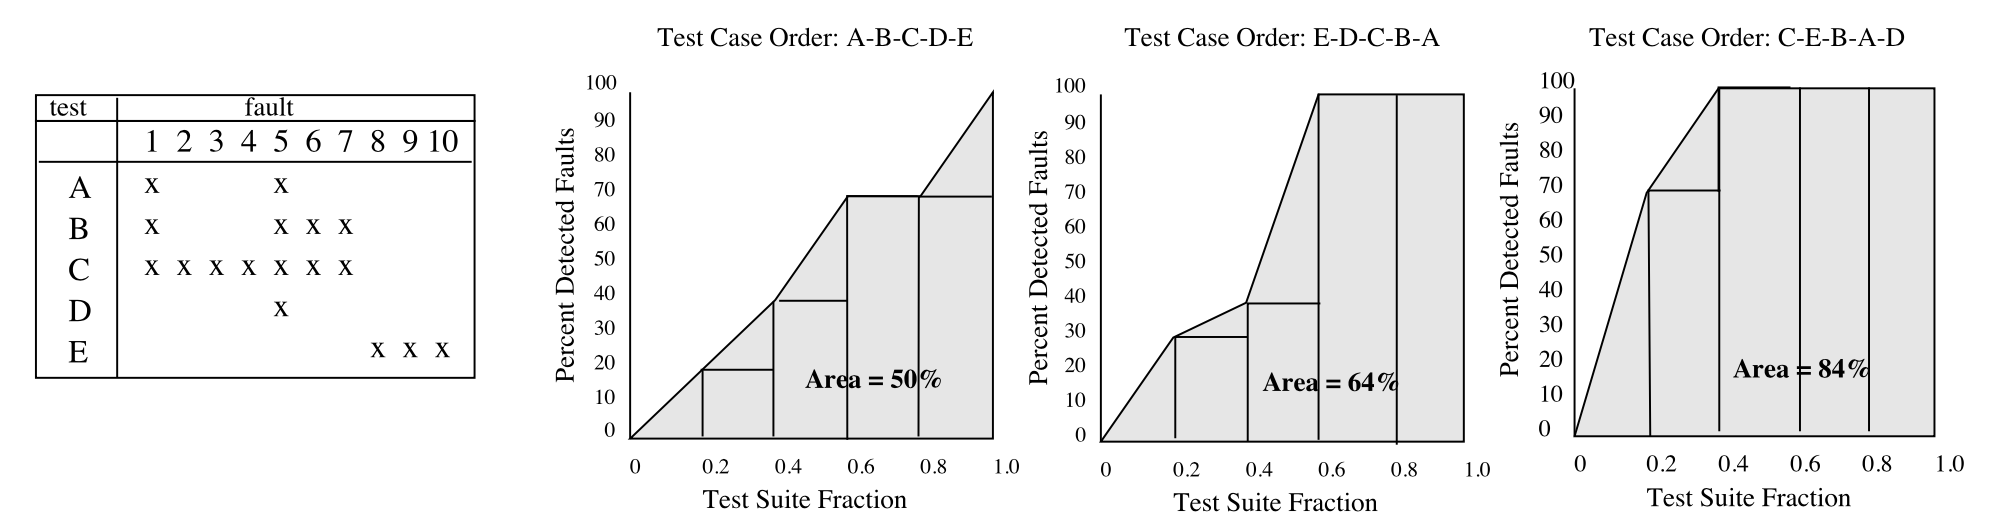
\includegraphics[scale=0.5, width=\linewidth]{figures/APFD.png}
	\caption{Average percentage of fault detection \cite{APFD}}
	\label{APFD}
\end{figure} 

The area below the plotted line is interpreted as the percentage of detected faults against the number of executed test cases, maximizing APFD, demonstrating clear results in detecting early applying fewer test cases. The order of test cases that maximizes APFD, with $ APFD = 84 \%$ is \textbf{C-E-B-A-D}, being preferable over other permutations.

By detecting faults early, the risk of developing over faulty code is reduced, causing minimal breakage in productivity avoiding, for example, possible delayed feature releases.\cite{Uber}

\section{Approach Exploration}

In this section, the goal is to provide a solid comparison between the different strategies that can be adopted to make sure source-code repositories are a manageable choice.

%-----------------------------------
%	SUBSUBSECTION 1
%-----------------------------------

\subsection{Naive-approach}

The simplest approach is to run every test for every single commit. As teams get bigger,  both the number of commits and the numbers of tests grow linearly, so this solution does not scale. Also, as \cite{Memon:2017:TGC:3103112.3103143} stated, computer resources grow quadratically with two multiplicative linear factors, making continuous integration a very expensive and not eco-friendly process in terms of resources and time.

For example, Google's source code is of the order of 2 billion lines of code and, on average, 40000 code changes are committed daily to Google's repository, adding to 15 million lines of code, affecting 250000 files every week, having the need to come up with new and innovative strategies to handle the problematic.\cite{Ziftci}


%-----------------------------------
%	SUBSUBSECTION 2
%-----------------------------------

\subsection{Cumulative Approach}

One possible solution to contour the large amount of time spent on testing and waiting for results is to accumulate all the commits made during working hours and test the last version, periodically, lets say during the night. This enables teams to develop at a constant speed without having the concern of breaking the master branch, but rather worrying about it in the future. In this case, the lag between making a commit and knowing if it passed or fail is very large, running the risk of stacking multiple mistakes on top of each other. 

Using this approach, two possible outcomes can occur: either the build passes every test and the change is integrated, or it fails, causing a regression. Here, we encounter another crossroads, as the batch was tested as a cumulative result, we have no information whatsoever of what commit, exactly, caused the regression. This problem can be solved by applying search algorithms:

\begin{itemize}
	\item \textbf{Binary Search} - instead of running every option, divide the list in half and test the obtained subset, if pass, the mistake is located in the other half, if fail, split the subset and test again until narrowing it down to a specific change, this approach is O(log n) complex.
\end{itemize}

After finding out which commit caused the regression, it can be fixed or rolled back to the version before the change was introduced, meaning that possibly the progress made during that working day has to be scrapped and re-done, postponing deadlines and, at a human level, lowering down motivation, with developers being "afraid" of making changes that will propagate and will only be detected later on, so allowing a large turn-around time may results in critical hampering of productivity.

In comparison with naive-approach, cumulative approach is more scalable in the way that it avoids testing every single commit made, only trying to test the last of the day, spending more time trying to trace back the origin of the failure. So in conclusion, we forfeit absolute correctness to gain speed and pragmatism, although this solution's computer resources grow linearly with the number and time of tests. 

The key here is that we should be able to go beyond finding items in a list were elements are interchangeable and equally informative. We should be able to use that information to do a much more efficient search. For example, we are looking for a faulty commit in a list of 10 elements and we know with a 95$\%$ probability that the commit is one of the last 4 elements, then we should only do binary search on those 4, instead of 10, thus saving time.

%-----------------------------------
%	SUBSUBSECTION 3
%-----------------------------------

\subsection{Change-List Approach}

In this case, changes are compiled and built in a serialized manner, each change is atomic and denoted as a Change List (CL). Clarifying, lets take a look at Google's example of workflow in Figure \ref{googleWF}.

\begin{figure}[H]
	\centering
	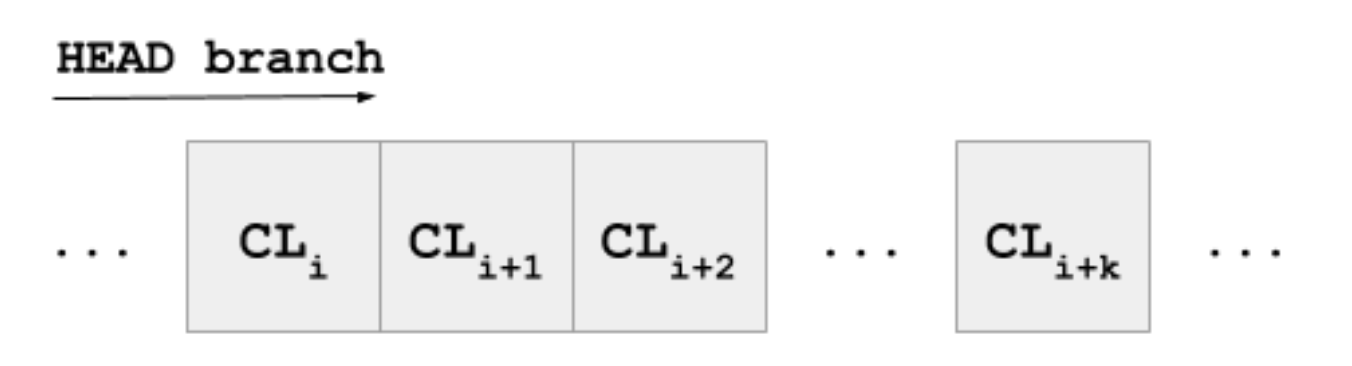
\includegraphics[scale=0.5, width=0.6\linewidth]{figures/Google_WorkFlow.png}
	\caption{Code repository and workflow at Google. Each CL is submitted to master branch or HEAD \cite{Ziftci}}
	\label{googleWF}
\end{figure} 

Individually, tests validate each CL and if the outcome is pass, the change is incorporated into the master branch, resulting into a new version of the code. Otherwise, a regression is caused. For example, imagine that $CL_i$ introduces a regression, causing failure on the consecutive system versions. Possible fixes and tips: investigate the modifications in $CL_i$, to obtain clues about the root cause of the regression; Debug the fail tests at $CL_i$, which is preferable to debug at later version $CL_{i+k}$, whereas after $CL_i$ code volume might increase or mutate, misleading conclusions; revert or roll back the repository, until the point where it was "green", in this case $CL_{i-1}$.\cite{Ziftci}


The novelty is introduced in test validation: 

\begin{itemize}
	\item \textbf{Presubmit tests} - Prior to CL submission, preliminary relevant small/medium tests are run, if all pass the submission proceeds, else it gets rejected. So instead of having to wait until all tests are complete, the developer has a quick estimate of the status of the project.
	\item \textbf{Postsubmit tests} - After CL submission, large/enormous tests are executed and if they indeed cause a regression, we are again in the situation where we have to find exactly what CL broke the build and, possibly, proceed in the same manner as Cumulative Approach to detect what version caused the regression. \cite{Ziftci}
\end{itemize}

Nevertheless there are some major issues: while presubmit testing, the sole focus is to detect flaws on individual changes and not on concurrent one. \textit{Concurrency} is the term referred to builds that run in parallel with each other, meaning that 2 developers can be committing changes of the same file, that are in conflict with each other, or with other files. Therefore, after precommit phase, there is the need to check all the affected dependencies of every commit, quickly identify were the conflict emerged and eventually roll back in the case of a red master, which can only be done in postcommit stage \cite{Uber} and when a postcommit test fails: a 45 minute test, can potentially take 7.5 hours to pinpoint which CL is faulty, given a 1000 CL search window, so automation techniques, quickly putting them to work and returning to a green branch is pivotal. \cite{Ziftci}

To better understand the concept of concurrency and the implications it brings, lets consider there are $n$ concurrent changes in a batch, where all of them pass precommit phase: (1) committing changes 1 to $n-1$ do not lead to breakage, (2) applying the $n^{th}$ change does not break the master, and (3) putting all the changes together breaks the mainline. Which might indicate that  the $n^{th}$ change is in conflict with the rest. Concurrency is practically unavoidable and it is more likely to happen when parts of the code that are interconnected are being altered. Frequent mainline synchronization is a possible path to diminish this effect, forcing developers to always work on the most updated version.\cite{Uber} 

%-----------------------------------
%	SUBSUBSECTION 4
%-----------------------------------

\subsection{Always Green Master Approach}

After steering clear of analysing every single change with every single test, or accumulating all the changes and testing them , splitting it into smaller individualized chunks, cherry-picking an ideal and non-redundant subset of tests, prioritizing them by size making it possible to divide test phase into precommit and postcommit, and enabling a status estimate of the likelihood of regressions,   \cite{Uber} proposes that an always green mainline is the priority condition, so that productivity is not hampered. To guarantee an always green master, Uber designed a scalable tool called \textit{SubmitQueue}, where every change is enqueued, tested and, only later on, integrated in the mainline branch if it is safe. The interesting aspect is which changes get tested first, while ensuring serializability. Uber resorts to a probabilistic model that can speculate on the likelihood of a given change to be integrated. - i.e. pass all build steps. Additionally, to agilize this process this service contains a \textit{Conflict Analyzer} to trim down concurrent dependencies. 

\subsubsection{Probabilistic Speculation} 

Based on a probabilistic model, powered by logistic regression, it is possible to have an estimate on the outcome a given change will have and with that information select the ones that are more likely to succeed, although other criteria might be chosen. To select the more likely to succeed changes, this mechanism builds a \textit{speculation tree}, which is a binary decision tree. Imagine a situation where two changes, $C_1$ and $C_2$, need to be integrated in the master branch $M$. $C_1$ is merged into $M$ is denoted by $M \oplus C_1$ and the build steps for that change are denoted by $B_1$. $B_{12}$ represents builds for $M \oplus C_1 \oplus C_2 $.  Speculating that $B_1$ has high probability of being integrated, it is useful to test it in parallel with $B_{12}$, because if the assumption is correct, $C_1$ is integrated and now this result can be used to determine if $C_2$ also passes, without testing each one individually and then together. If the speculation is not correct, $C_1$ is not merged and $C_2$ has to build separately by running $B_2$. In the case of three pending changes $C_1$,$C_2$ and $C_3$, the speculation tree is of the form of Figure \ref{spectree}. One possible way of handling the result from this tree would be to speculate everything, assuming that the probability of merging a change is equal to the probability of rejecting it. Having 3 pending changes, one would have to perform 7 builds (number of nodes in the tree), under this assumption. But it is unnecessary to speculate all of the builds, if $B_1$ is successful, $B_2$ now becomes irrelevant and the tree is trimmed down considerably. Only $n$ out of $2^n - 1$ builds are needed to commit $n$ pending changes \cite{Uber}. Additionally, the assumption that every change depends on one another is made, but this is not always the case, two changes can be totally distinct. By detecting independent changes,  a lot of time can be saved by building them individually and committing them in parallel. This is done by the Conflict Analyzer. This approach combining the selection of most likely to pass builds, using machine learning models, parallel execution, the identification of independent changes, trimming down speculation tree size is able to scale thousands of daily commits to a monolithic repository. Finally, a comparison of all explored approaches is shown in the Table below.


\begin{figure}[H]
	\begin{floatrow}
		\ffigbox{%
			\centering
			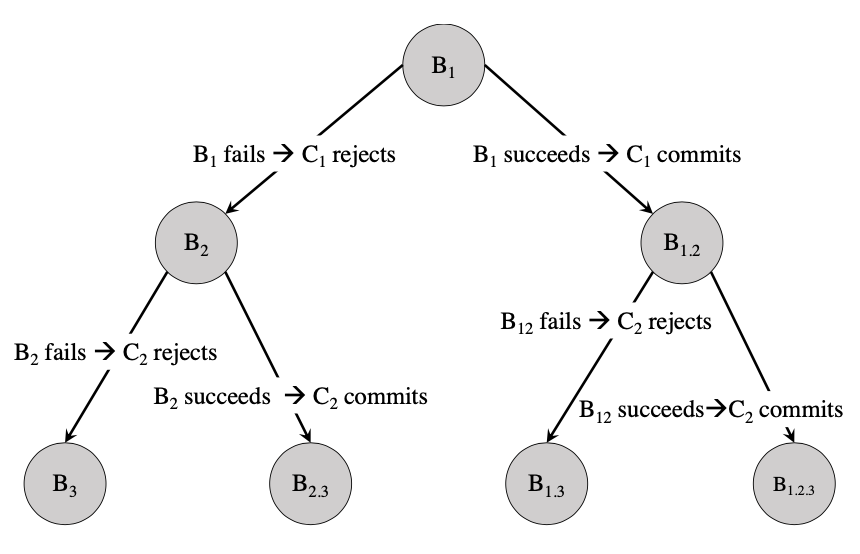
\includegraphics[scale=0.5, width=\linewidth]{figures/spectree.png}
		}{%
			\caption{Speculation tree - builds and outcomes \cite{Uber}}
			\label{spectree}
		}
		\capbtabbox{%
			\resizebox{.5\textwidth}{!}{
				\begin{tabular}{lccc}
					\hline
					\textbf{Approach} & \multicolumn{1}{l}{\textbf{Correctness}} & \textbf{Speed}    & \multicolumn{1}{l}{ \textbf{Scales?}} \\ \hline
					Naive                & Very High                       & Very Low & No                                   \\
					Cumulative           & Medium                          & Low      & No                                   \\
					Change-List          & Medium                            & Medium     & Yes                                  \\
					Always Green Master  & High                            & High     & Yes                                  \\ \hline
				\end{tabular}
				\caption{Comparative analysis between strategies}}
		}{%
			
		}
	\end{floatrow}
\end{figure}

%%%%%%%%%%%%%%%%%%%%%%%%
%%%%%%%%%%%%%%%%%%%%%%%%

\section{Machine Learning}

Machine Learning algorithms are at the forefront in achieving effective automatic regression testing. By building predictive models, it is possible to accurately, and most importantly, quickly, identify if a newly introduced change is defective or not. This helps developers to check and amend faults, when the details still remain fresh on their minds and it allows to prioritize and organize changes by the risk of being defective, this way testing the ones that are more likely to fail first, diminishing the lag-time between committing and feedback.

In recent years, several researchers studied the usefulness of applying fault-prediction techniques , powered by machine learning algorithms. %citation
More concretely, resorting to an emergent area which is Deep Learning. Kamei et. al propose an approach called \textit{Deeper}, that is divided into two phases: the feature extraction phase and the machine learning phase. The first consist on identifying a combination of relevant features from the initial dataset, by using Deep Belief Networks. The latter is encapsulated on building a classifier/predictive model based on those same features.

In this work, the author aims to replicate and explore the techniques developed by ... and ..., extending the domain of validity and achieving higher levels of accuracy, by experimenting other classifiers and feature extraction techniques.

In the next sections, a theoretical background will be elaborated on the several techniques used throughout the thesis, to provide a solid base for moving forward.

\section{Supervised Learning}

Supervised Learning is the task of learning by example and it is divided into a training phase and a testing phase. In the first, the learner receives labelled data as input and the output is calculated, then based on a cost function that relates the predicted value with the actual value, the parameters of the model are updated such that the cost function is minimized. Then, in the second phase, the model is tested with new data, that it has never seen before, and its performance is evaluated. 
Supervised Learning can be divided into two groups: Classification and Regression. In classification, each item is assigned with a class or category, e.g. if an email is considered spam or not-spam, represents a binary classification problem. Whereas in regression, each item is assigned with a real-valued label. \cite{HanDataMining}


In accordance with Kamei et al. \cite{kameiJIT} and Yang et al. \cite{yangJIT}, the typical predictive model used is the Logistic Regression. Here, other models are explored, such as Decision Trees, Ensemble Methods and Artificial Neural Networks.

\subsection{Logistic Regression}

In classification, the goal is to come up with a rule to guess an outcome from a set of input variables. More precisely, when the output is binary, i.e. there are only two classes, this rule will predict, for example, if it will rain tomorrow, or not; or if a patient has a certain disease, or hasn't; or if the house mortgage will be payed, or not. Nonetheless, providing a "yes" or "no" answer to every observation is a quite rough estimate. - this type of classifiers are of type "hard" \cite{ml_phys}. Especially in the presence of noisy data, adopting a "softer" approach to incorporate such nuances would be useful: like determining the probability that each data point has of being "0" or "1", rather than a binary output.\cite{shalizi} Logistic Regression corresponds to the corner stone of "soft" classifiers, which are, sometimes, more useful to resort to. There are situations where it is much more useful to know the likelihood/risk of something, instead of the actual values, thus having the possibility to rank observations in the most convenient way. \cite{ml_phys}
For example, an international bank desires to investigate which customers are more likely to leave. Considering certain features, like age, gender, country, number of credit cards, amount of debt, credit score, etc, the bank can train a model based on past history, to apply to customers that the model has not "seen" and rank them by risk. Using such information to adapt and prioritize actions on customers that are more likely to leave. 

To sum up, for a binary output variable $Y$, one needs to model the conditional probability $P(Y=1|X=x)$ as function of $x$. A good starting point would be to try to do it by using a simple \textit{linear regression}: (1) At first glance, one possible solution would be to let $p(x)$ be a linear function of $x$. An increment on the value of x would reflect on adding or subtracting a certain quantity to the probability. The drawback comes from the unboundedness of linear functions, and probabilities are bound between 0 and 1. (2) To solve the boundary problem, one can let $log$ $p(x)$ be a linear function of $x$. Incrementing the value of $x$, will multiply the probability by a fix amount. But logarithms are only bounded in only one direction. (3) Finally, the most straight forward modification of (2) is the \textbf{logistic transformation}, $log(\frac{p}{1-p})$, which bounds the probability from $0$ to $1$, not compromising the interpretability of the result. \cite{shalizi}.


Let $x_i = \{x_1 , x_2 , ...x_m \}$ is defined as the vector representation of features of a data point $x$, and $x_i$ represents the value of the $i-th$ feature of $x$, and $W = \{w_0, w_1, w_2, ...w_m\}$ denotes the weight vector associated to the features in $x$, $w0$ is a bias parameter, and $w_i, i \in \{1, 2, ...m\}$ is the weight of the $i-th$ feature of $x$ (i.e., $x_i$ ), and the let $y_i = \{y_1 , y_2 , ...y_m \}, y_i \in \{0,1\}$ be the observed class.

Formally, the logistic regression model is given by:
\begin{equation}
y = log\bigg(\frac{p(x)}{1-p(x)}\bigg) = w_0 + x \cdot w 
\end{equation}

Solving for $p$, yields:

\begin{equation}
p(x,w_0,w) = \frac{e^{w_0 + x \cdot w }}{1+e^{w_0 + x\cdot w }} = \frac{1}{1 + e^{-(w_0 + x \cdot w )}}
\end{equation}

\begin{equation}
p(y=1) = 1 - p(y=0) 
\end{equation}

Now, what is left is to estimate the parameters $w_0$ and $w$ and this can be achieved by maximizing the likelihood function, so that the obtained statistical model best fits the observed data. 
The probability of an observed class $y_i$ is either $p$, if $y_i = 1$, or $1-p$, if $y_i = 0$. Then the likelihood is: 

\begin{equation}
L(w_0,w) = \prod_{i=1}^{n} p(x_i)^{y_i}(1-p(x_i))^{1-y_i} 
\end{equation}

For convenience, it is usual to write the \textit{log-likelihood}: $log\bigg(L(w_0,w)\bigg)$:


\begin{align} 
l & = \sum_{i=1}^{n} y_i log(p(x_i))+(1-y_i)log(1-p(x_i)) \\
& = \sum_{i=1}^{n} log(1-p(x_i)) + \sum_{i=1}^{n} y_i log(\frac{p(x_i)}{1-p(x_i)}) \\
& = \sum_{i=1}^{n} log(1-p(x_i)) + \sum_{i=1}^{n} y_i(w_0 + x_i \cdot w) \\
& = \sum_{i=1}^{n} - log(1 + e^{-(w_0 + x \cdot w )} ) + \sum_{i=1}^{n} y_i(w_0 + x_i \cdot w)
\end{align}

Now, to maximize the log-likelihood, one differentiates $l$, with respect to its parameters $w_i$. Differentiating with respect to one specific parameter $w_j$, the result obtained is:

\begin{align}
\frac{\partial l}{\partial w_j} & = -  \sum_{i=1}^{n} \frac{1}{1 + e^{-(w_0 + x \cdot w )}}e^{-(w_0 + x \cdot w )}x_{ij} +   \sum_{i=1}^{n} y_i x_{ij} \\
 & = \sum_{i=1}^{n} \bigg( y_i - p(x_i,w_0,w) \bigg)x_{ij}
\end{align}

Equalling the expression to zero and solving for $w_j$ would return the optimized value for the parameter, however this equation cannot be solved analytically, only by a numerical approximation \cite{shalizi}  The determination of the optimal parameters is what characterizes the training part of the algorithm. 


\subsection{Decision Trees}

Another potential candidate to treat our data may be a Decision Tree Classifier, which is categorized by having a flowchart-like tree structure, where there are nodes and branches. Each internal node denotes a test on an attribute and the branch represents the outcome of that test, then the nodes at the bottom of the tree, called \textit{leaf-nodes} whereas the topmost node is the \textit{root-node}, holds a class label. An example of such tree can be seen below\cite{HanDataMining}:

\begin{figure}[H]
	\centering
	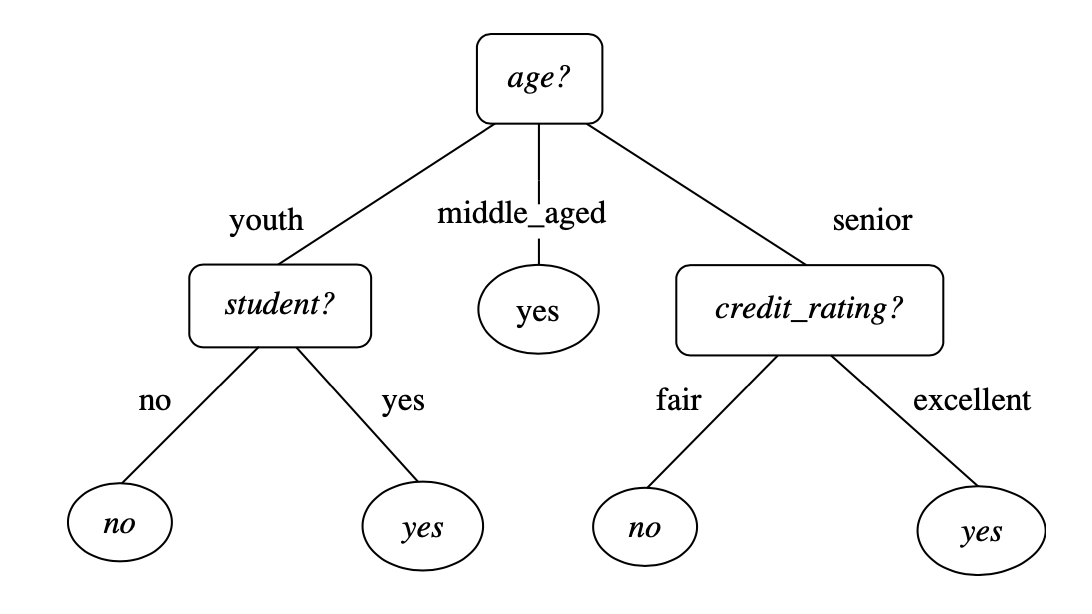
\includegraphics[scale=0.5, width=0.6\linewidth]{figures/DecisionTreeDiagram.png}
	\caption{Each internal (non-leaf) node represents a test on an attribute. Each leaf node represents a class (if the client is likely to buy the product yes/no )}
	\label{DTDiagram}
\end{figure} 

Then after training, when a new element serves as input of a Decision Tree, a path is traced from the root until the leaf node, revealing the prediction of which class that element belongs. Decision tree learning can be based in several algorithms. The most commonly used are ID3 ( Iterative Dichotomiser 3) , C4.5 and CART (Classification and Regression Trees). In this work, the chosen algorithm is provided by the \textit{scikit-learn} package and it uses an optimized version of CART. The mathematical formulation is as follows: 

\subsubsection{Mathematical formulation}

Given training vectors $x_i \in \Re^n, i = {1 , ... m} $ and a class label vector $y \in \Re^m$, a decision tree recursively partitions the space such that the samples equally labeled are grouped together. 

Considering the data at node $l$ be represented by $D$. For each candidate split $Q= (j, t_l),$, where $j$ corresponds to the \textit{j-th} feature and $t_m$ the threshold, partition the data into the subsets $D_{left}(\theta)$ and $D_{rigth}(\theta) $.

\begin{align}
D_{left}(\theta) &= (x,y) | x_j \le t_l \\
D_{right}(\theta) &= D \ D_{left}
\end{align}

Then, because data is not easily separable,i.e. partitions not often contain elements with the same class label, one defines a criterion called \textit{impurity}, that measures the probability of finding a mislabelled element in the subset. The impurity at $m$ is determined by using an impurity function $H()$, that depends if the task is classification or regression. 

\begin{equation}
G(D,\theta) = \frac{n_{left}}{N_l}H(G(D_{left},\theta)) + \frac{n_{right}}{N_l}H(G(D_{right},\theta)) 
\end{equation}

where $n_{left}$ is the number of attributes partitioned to the left, $n_{right}$ to the right and $N_m$ the total number of attributes in a node. The function H() is commonly defined \\

as Gini Impurity: 
\begin{equation}
	H(D_m) = \sum_k p_{mk}(1-p_{mk})
\end{equation}

as Entropy:
\begin{equation}
H(D_m) = -\sum_k p_{mk}(log(p_{mk})
\end{equation}

where $p_{mk}$ is the probability that an item $k$ with label $m$ is chosen.

The goal is to select parameters such that the impurity is minimised, such that:

\begin{equation}
\theta^* = argmin_{\theta}  G(D, \theta)
\end{equation} 

Finally, recursively apply the same reasoning to subsets $D_{left}(\theta^*)$ and $D_{right}(\theta^*)$, until maximum tree depth reached, i.e. $N_m < min_{samples}$ \cite{DTform}

\subsection{Ensemble Methods}

An ensemble combines a series of k learned models (or base classifiers), M1, M2,..., Mk, with the aim of creating an improved composite classification model, $M_{*}$.  

Ensemble methods are powerful tools for classification, namely \textit{random forests} and \textit{boosting}. An ensemble takes into account a series of $k$ learned models $M_1, M_2,...,M_k$, intersecting them into one,  more robust, model $M_*$. A good analogy is to think of decision trees as having medical diagnosis from one doctor, that enquires and measures the patient's symptoms and then draws a conclusion. Now, ensembles take into consideration the opinion of several doctors and decides based on this information. 

In this work, the ensemble method chosen is the Random Forest Classifier, that is an estimator that fits a various numbers of decision trees. \cite{HanDataMining}

to be continued

\subsection{Artificial Neural Networks}

In general terms, a neural network(NN) is a set of connected input/output units in which each connection has a weight associated with it. The weights are adjusted during the learning phase to help the network predict the correct class label of the input vectors.

In light of the knowledge psychologists and neurobiologist have on the structure of the human brain, more precisely on how neurons pass information to one another, this way it was possible to look for methods to develop and test computational analogues of neurons. Generally, a NN is defined as a set of input/output \textit{units} (or \textit{perceptrons}) that are connected. Each connection has a weight associated with it, and these weights are adjusted in such manner, that the network is able to correctly predict the class label of the input data. The most popular algorithm for NN learning is \textit{back-propagation}, which gained popularity since 1980. \cite{HanDataMining}

Usually, NN training phase involves a long period of time and a several number of parameters have to be set to build the network's structure and architecture. However, there is no formal rule to determine their optimality and this is achieved empirically, by running different experiments. This, nonetheless, raises an issue of poor interpretability, that makes it hard for humans to grasp what the optimal parameters mean. 
On the other hand, NN's compensate on easy-going implementation and ability to deal with noisy data and, so far, have been used to solve many real-world problems, such as hand written text recognition, medical diagnosis and finance. \cite{HanDataMining}

In the following sections, the reader is guided in detail through the architecture of a NN and given a brief explanation of how back-propagation works.

\subsubsection{Perceptron}

A perceptron is the most elementary unit of a NN. In similarity to brain cells, that are composed by dendrites, that receive electric signals (input), the nucleus that processes them and the axon, that sends too an electric signal to other neurons (output). In our case, the perceptron receives a vector of inputs ${x_1, x_2,... x_n}$ and associated to each one there are weights ${w_1,w_2,...w_n}$ that symbolize the influence each input has on the output. As an example, consider a perceptron with an input vector composed of 3 inputs ${x_1, x_2, x_3}$.

\begin{figure}[H]
	\centering
	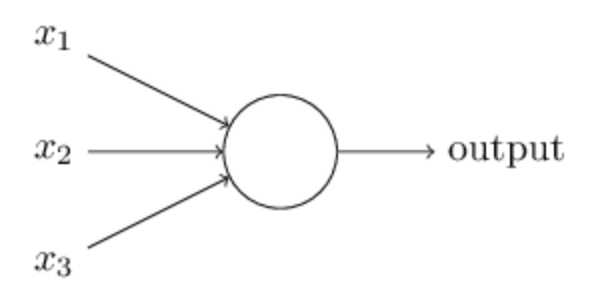
\includegraphics[scale=0.5, width=0.35\linewidth]{figures/perceptron.png}
	\caption{Perceptron simple example)}
	\label{perceptron}
\end{figure} 

 Let us say the desired output is either $0$ or $1$. This value shall be determined by weighing the sum $ \sum_j w_j x_j$ and checking if the value surpasses a given threshold \cite{nielsenneural}. So the output can be defined as: 

\begin{equation}
\mbox{\textbf{output}} = \begin{cases} 0, & \mbox{if } \sum_j w_j x_j \le \mbox{ threshold} \\ 1, & \mbox{if } \sum_j w_j x_j > \mbox{ threshold} \end{cases}
\end{equation}

Also, one can replace $ \sum_j w_j x_j$ as the dot product $w \cdot x $ and move threshold to the other side of the equation and call it $b$, for bias.

 \begin{equation}
 \mbox{\textbf{output}} = \begin{cases} 0, & \mbox{if } w \cdot x + b \le 0 \\ 1, & \mbox{if }  w \cdot x + b > 0 \end{cases}
 \end{equation}

Here, the bias term can be thought as the susceptibility of the neuron being activated, the large the value of $b$, more easily the output is 1. 

\subsubsection{Activation Functions}
There is a problem related to the sensitivity the perceptron has when $w \cdot x + b $ is close to zero. Small changes in the weights may cause a drastic effect on the outcome, because the expression corresponds to a step function. What can be done is define an activation function $\sigma(z)$ that transforms the expression above. Commonly,  $\sigma(z)$ is defined as the sigmoid function $\sigma(z) = \frac{1}{1+e^{-z}}$ , or the rectifier function $\sigma(z) = max(0,z) $, comparing the three curves for the same values of $w_i$ and $b_i$:

\begin{figure}[H]
	\centering
	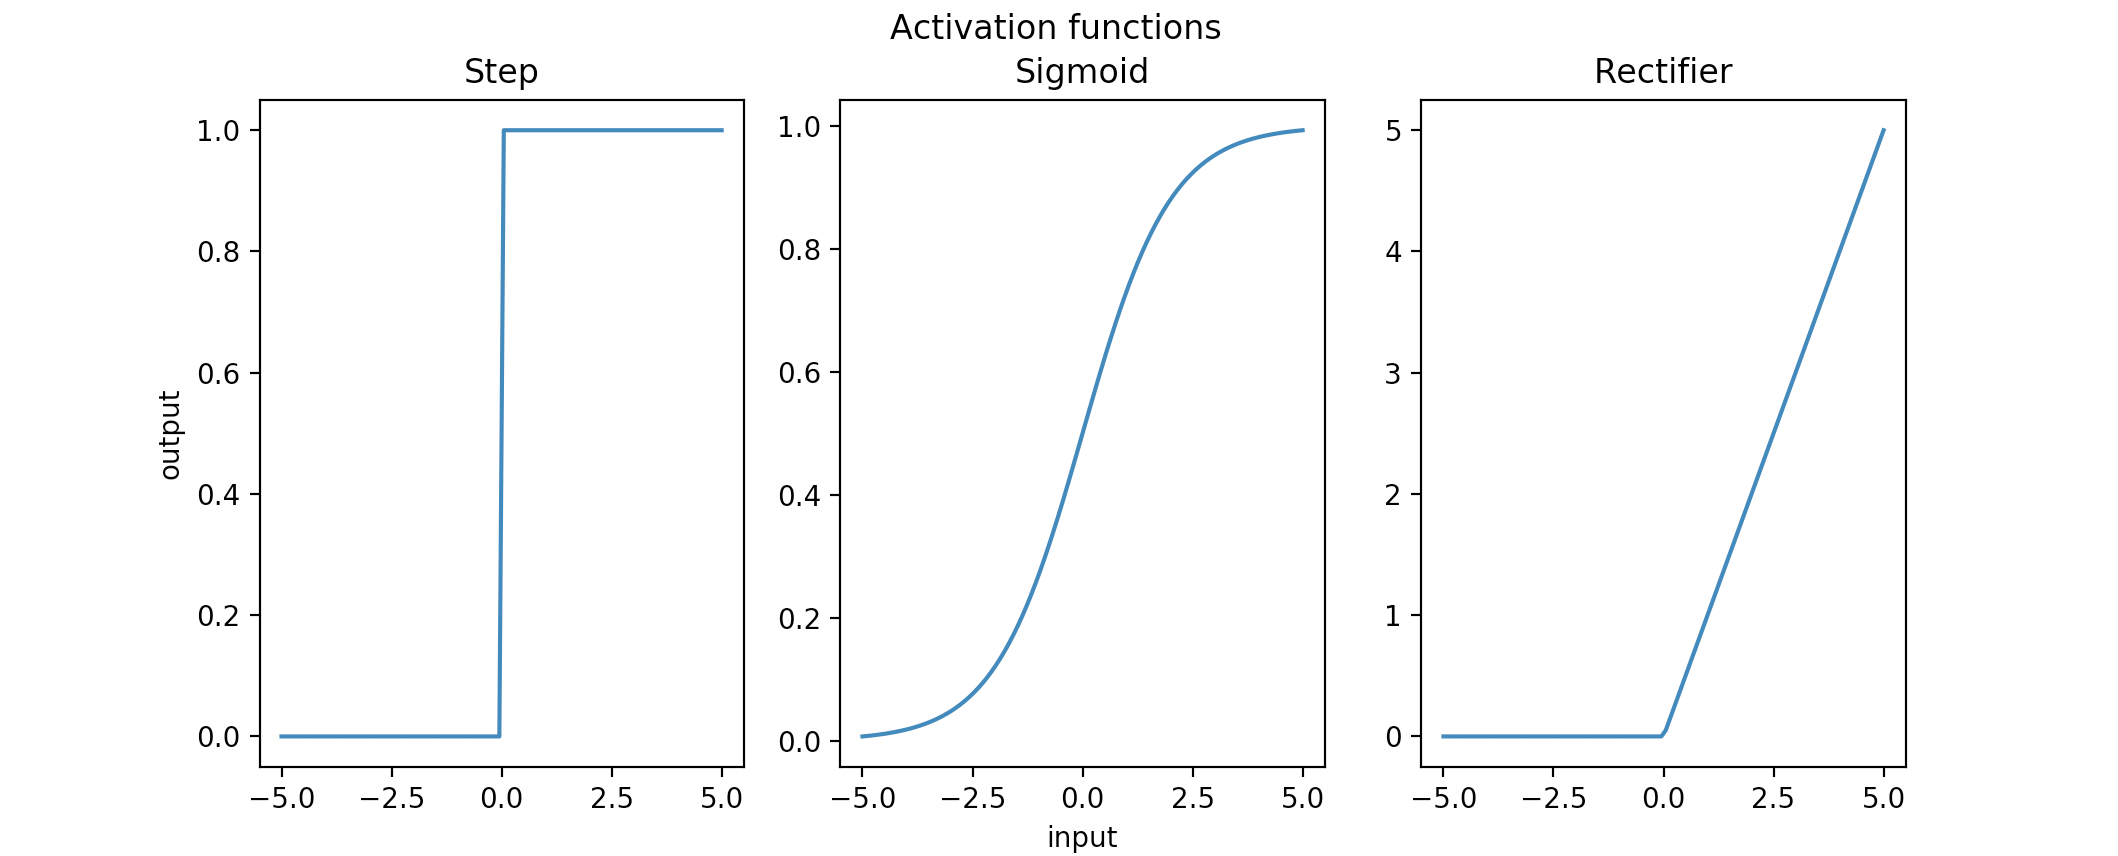
\includegraphics[scale=1, width=\linewidth]{figures/activationfunc.png}
	\caption{Comparative analysis of different activation functions (made in Python))}
	\label{perceptron}
\end{figure} 
In the first image, the transition from 0 to 1 is abrupt and steep, this way values that are close to the threshold can have dramatic distinctions in output and that is not desirable, because NN's learn by making little adjustments on the values of the weights. By using the sigmoid function values are smoothed out in a way that values no longer have a binary outcome, but rather a continuous and  progressive approximation to the values zero or one. For high positive inputs, the output is very close to one, the same happens for high negatives close to 0 (like in the step function case) and in between the curve is softer, also the sigmoid function in differentiable in all its domain. The third case corresponds to the rectifier function that only activates for positive values and due to its easy implementation, its usage because relevant in reaching high performance.

\subsubsection{NN architecture }

Now, very much alike the human brain, perceptrons are assembled together to form a connected structure called a network. By grouping perceptrons of the same type. - input, output or neither.- layers are form and there are three types: input layer, output layer and \textit{hidden} layer. The neuros that belong to the hidden layer are simply neither input nor output neurons, they serve as a mean of adding more complex relations between the variables input and weights. In terms of configuration, there is only one input layer and one output layer, with variable size. However multiple hidden layers may exist. Let us take the following example with an input vector of size $6$, an output vector with size $1$ and $2$ hidden layers of size $4$ and $3$. \cite{nielsenneural}.


\begin{figure}[H]
	\centering
	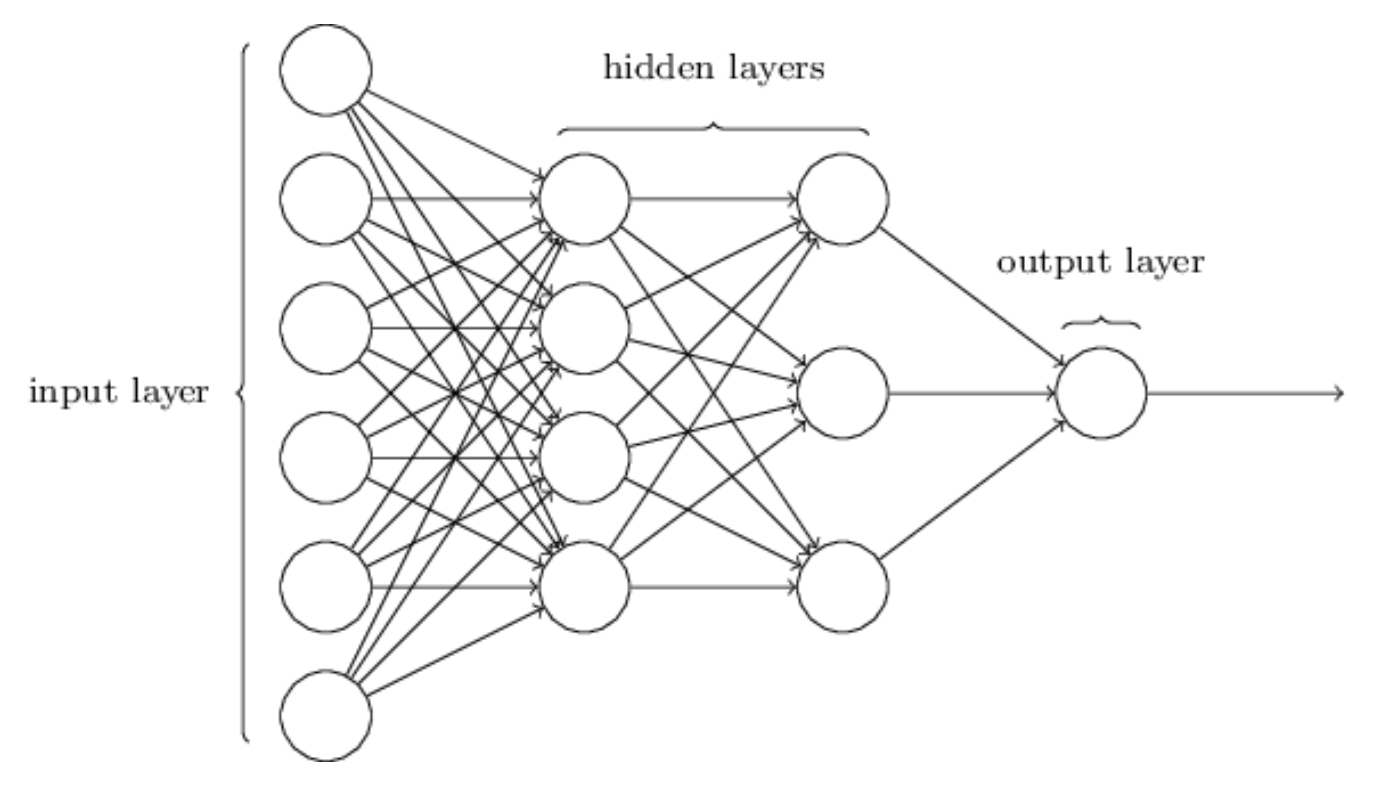
\includegraphics[scale=0.5, width=0.65\linewidth]{figures/nnarch.png}
	\caption{Architecture example of a NN \cite{nielsenneural}}
	\label{nnarch}
\end{figure} 

Every node as a connection to a node from the next layer, but what is changeable is the number of hidden layers and the number of nodes in each layer. Although there are some heuristics to determine the best configuration.- like choosing the number of neurons by averaging the number of neurons in the input and output layer.-  each dataset has its own characteristics, it becomes difficult to come up with a rule of thumb that works in generality, so one has to determine the parameters by running experiments.\cite{nielsenneural}

To wrap up the functioning of a NN,  from an input vector $x$, the neurons from the next layer will be activated or not by computing $w \cdot x + b$, then the same process occurs until the output node is reached, in this case yielding the result $1$ or $0$, this left-to-right process is called \textit{forward-propagation}. Of course, this is not the process of learning, most likely if one compares the predicted result with the actual value, it is a $50 \%$ chance of being correct. So how does a NN learn?

\subsubsection{Learning with Gradient Descent}

As mentioned above, the desired result is achieved once the difference between the predicted value $\hat{y}$ and the actual actual $y$ is minimized. The goal is to find an algorithm that will indicate which values for weights and biases will produce the correct output. In order to quantify the performance achieved so far, let us define a cost function $C(Y,\theta)$,where in the  dataset $Y$, $\theta$ are the parameters, , $m$ the total number of samples in the dataset and $i$ its index.:

\begin{equation}
 	C(Y,\theta) = \frac{1}{2m}\sum_{i=1}^{m}(\hat{y}^{(i)} - y^{(i)})^2
\end{equation}

In this formula, one sees that it is close to zero, exactly when the predicted value matches the expected value. A possible approach to reach this result could be to brute force the values of the parameters: trying out several combinations of weights and biases, narrowing down in each iteration, eventually converging towards the quadratic value, or the minimum of the cost function. However, this approach does not scale. With just $25$ weights and assuming each weight can have $1,000$ different values, there are $1000^{25} =10^{75}$ possible combinations, which is infeasible to compute, even for modern supercomputers\cite{ml_phys}.
A more efficient strategy is to use Gradient Descent to minimize the cost function. The first step would be to randomly initialize all the weights and bias, similar to the initial condition of a differential equation, and then calculate the output $\hat{y}$ and compute the cost function. Most likely, it will not yield a result close to the minimum, so now one needs to know is what direction of the curve points towards the minimum and then "jump" a step towards that direction. This is achieved by calculating the gradient of the cost function, with respect to $\theta$.
\begin{align}
	v_t &= \eta_t \nabla_{\theta} C(Y,\theta) \\
	\theta_{t+1} &= 	\theta_{t}  - v_t
\end{align}

where  $\eta_t$ is the \textit{learning rate} that defines the length of the step taken in the direction of the gradient , at time step t. By configuring a small learning rate it is guaranteed local minimum convergence, however implying a high computational cost and not assuring an optimal solution by landing on a global minimum. On the other hand, by choosing a large learning rate the algorithm can become unstable and overshoot the minimum. (possible oscillatory dead-end).\cite{ml_phys}.  Minimising a cost function looks this:

\begin{figure}[H]
	\centering
	\begin{minipage}{.5\textwidth}
		\centering
		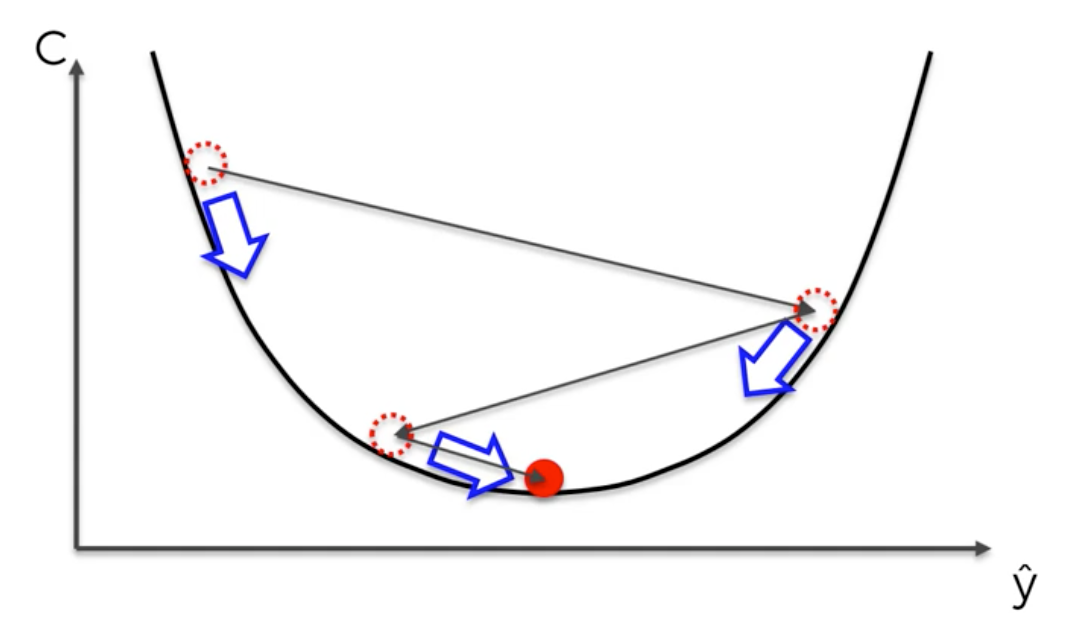
\includegraphics[width=.9\linewidth]{figures/graddesc.png}
		\label{fig:test1}
	\end{minipage}%
	\begin{minipage}{.5\textwidth}
		\centering
		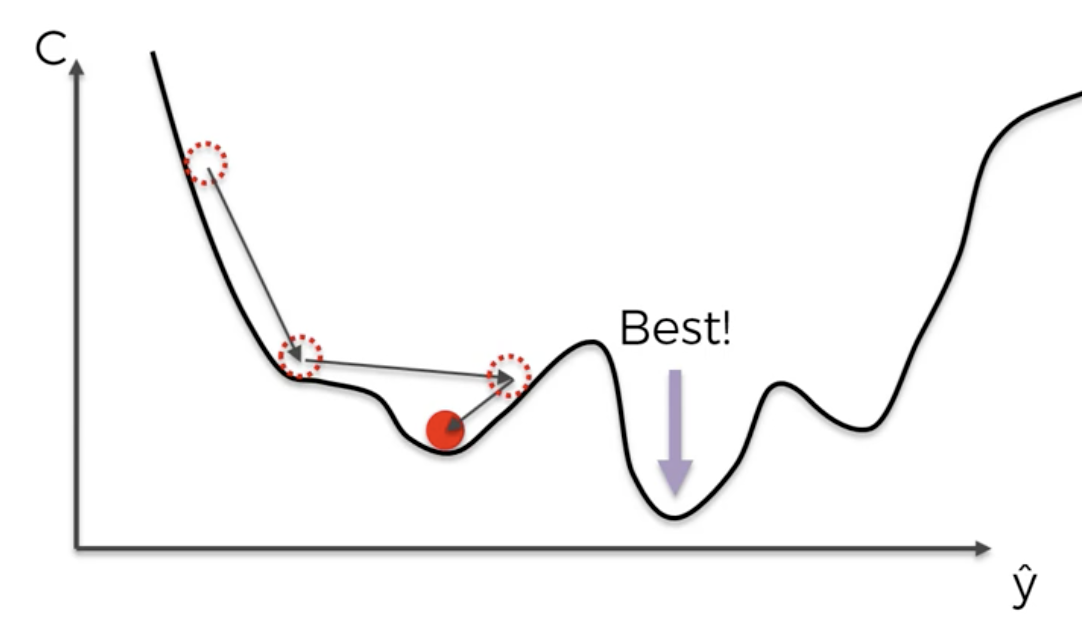
\includegraphics[width=.9\linewidth]{figures/graddesc2.png}
		\label{fig:test2}
	\end{minipage}
	\caption{Global and Local minimum determination \cite{udemyDS}}
\end{figure}

In this one dimensional example, the gradient yields the direction towards the minimum and the learning rate determines the length of the step. However, in the second case, there are some cases where convergence is sub-optimal. This information hints the conclusion that choosing simple gradient descent, as our minimizing algorithm, has many limitations, namely:

\begin{itemize}
	\item \textit{Finding global minimum} - only local minimum are guaranteed to be found under the gradient descent algorithm.
	\item \textit{Sensitive to initial conditions} - depending on the starting point, the final location most likely will be a different minimun, hence there is a high dependency on initial conditions.
	\item \textit{Sensitive to learning rate} - as seen above, learning rate can have a huge impact on the algorithm's convergence.
	\item \textit{Computationally expensive} - although better than brute force, when handling large datasets, computation rapidly increases cost. Possible solution is to just apply the algorithm to a subset or \textit{"mini-batch"}
	\item \textit{Isotropic parameter-space} - Learning rate is always the same independent of the "landscape". Ideally, the learning rate should be larger in flatter surfaces and smaller in steeper ones. \cite{ml_phys} 
\end{itemize}
 

\subsubsection{Stochastic Gradient Descent (SGD)}

To handle the limitations described in the section above, a novel, more efficient algorithm is proposed: the Stochastic Gradient Descent (SGD). The advantage is that, not only the method is more computationally efficient, but it also deals with non-convex cost-functions, on the contrary of simple gradient descent, also called \textit{batch} gradient descent method, because it plugs every item of the dataset into the neural network, obtains the predicted values, calculates the cost function by summing the square differences to the expected value and only then the weights are adjusted. \cite{nielsenneural}
SGD works in a different way, here the batch is divided into $n/M$ subsets or \textit{mini-batches} $B_k, k={1,...,n/M}$, where $n$ is the total number of data points and $M$ the mini-batch size. The gradient now takes the following form: 

\begin{equation}
\nabla_{\theta} C(Y,\theta) = \frac{1}{2m}\sum_{i=1}^{n}\nabla_{\theta} (\hat{y}^{(i)} - y^{(i)})^2 \rightarrow \frac{1}{2m}\sum_{i \in B_k}\nabla_{\theta} (\hat{y}^{(i)} - y^{(i)})^2
\end{equation}


Each mini-batch $B_k$ is plugged into the NN, the cost function is calculated and the weights are updated. This process repeats $k$ times until the whole data set is covered. A full run over all $n$ points is denoted as an \textit{epoch}. \cite{ml_phys}

In sum, SGD has two very important advantages: not only eliminates the local minimum convergence problem, by introducing stochasticity , but also it is much more efficient in computational power, because only a subset of $n$ data points has to be used to approximate the gradient.


\subsubsection{Backpropagation}

So far, a review of the basic structure and training of NN has been provided: starting from the elementary unit.- the perceptron - up to how many of them can be assembled, covering the most common types of activation functions. Then the concept of forward propagation was introduced along with a cost function that allows to judge whether the model created explains the observations. The goal is to minimise the cost function, resorting, in a first approach, to the gradient descent method which, as seen above, has severe limitations, concluding that the Stochastic Gradient Descent algorithm is most suited for this task. However, SGD still requires us to calculate the derivative of the cost function with respect to every parameter of the NN. So a forward step has to be taken to compute these quantities efficiently. - via the \text{backpropagation} algorithm. - to avoid calculating as many derivatives as there are parameters. Also backpropagation enables the determination of the contribution of each weight and bias to the cost function, altering more, the weights and biases that contribute the most, thus understanding how changing these particular values will affect the overall behaviour. \cite{nielsenneural}

The algorithm can be summarized into four equations, but first, let us define some notation. Assuming a network composed of $L$ layers with index $l = {1,... L}$ and denote by $w_{j,k}^l$ the weight connecting from the \textit{k-th} neuron of layer \textit{l-1} to the \textit{j-th} neuron in layer \textit{j}. The bias of this neuron is denoted $b_l^j$. By constructing, one can write the activation function $a_j^l$ of the  \textit{j-th} neuron in the  \textit{l-th} layer, by recursively writing the relation to the activation $a_j^{l-1}$ of neurons in the previous layer \textit{l-1}.

\begin{equation}
a_j^l = \sigma\bigg(\sum_{k}\omega_{j,k}^l a_k^{l-1} + b_j^{l} \bigg) = \sigma(z_j^l)
\label{first}
\end{equation}

When calculating the cost function $C$, one only needs to take directly into account the activation from the neurons of layer $L$, of course the influence of the neurons from previous layers is underlying. So one can define the quantity, $ \Delta_j^L$, which is the error of the \textit{i-th} neuron in layer L , as the change it will cause on the cost function $C$, regarding weighted input $z_j^L$:

\begin{equation}
\Delta_j^L = \frac{\partial C}{\partial z_j^L}
\end{equation}
Generally, defining the error of neuron $j$ of any layer $l$ and applying the chain rule to obtain the first equation of the algorithm:

\begin{equation}
\Delta_j^l = \frac{\partial C}{\partial z_j^l} =  \frac{\partial C}{\partial a_j^l} \frac{\partial a_j^l}{\partial z_j^l} =  \frac{\partial C}{\partial a_j^l} \sigma '(z_j^l)
\label{backprop1}
\end{equation}

Now, one can relate the error function $ \Delta_j^L$ to the bias $b_j^{l}$ to obtain the second backpropagation relation:

\begin{equation}
\Delta_j^L = \frac{\partial C}{\partial z_j^L} = \frac{\partial C}{\partial b_j^l} \frac{\partial b_j^l}{\partial z_j^l} = \frac{\partial C}{\partial b_j^l}
\label{backprop2}
\end{equation}

Since, $\frac{\partial b_j^l}{\partial z_j^l} = 1$ , from \ref{first}. 
Furthermore to find another expression for the error, one can relate the neurons in layer $l$ with the neurons in layer $l+1$: 

\begin{align}
\Delta_j^l &= \frac{\partial C}{\partial z_j^l} = \sum_k \frac{\partial C}{\partial z_k^{l+1}} \frac{\partial z_k^{l+1}}{\partial z_k^{l}} \\
&= \sum_k  \Delta_k^{l+1}  \frac{\partial z_k^{l+1}}{\partial z_k^{l}} \\
&= \bigg( \sum_k  \Delta_k^{l+1} \omega_{k,j}^{l+1}\bigg) \sigma '(z_j^l)
\label{backprop3}
\end{align}


This is the third relation. Finally, to derive the final equation, one differentiates the cost function with respect to the weights $\omega_{j,k}^l:$

\begin{equation}
\frac{\partial C}{\partial \omega_{j,k}^l} =\frac{\partial C}{\partial z_{j}^l}\frac{\partial z_{j}^l}{\partial \omega_{j,k}^l} = \Delta_j^{l} a_k^{l-1}
\label{backprop4}
\end{equation}

The combination equations \ref{backprop1}, \ref{backprop2}, \ref{backprop3} and \ref{backprop4}, constitutes the backbone of the backpropagation algorithm that is used to train NN's in a very efficient way \cite{ml_phys}. It described in the following steps:

\textbf{Backpropagation Algorithm:}
\begin{enumerate}
	\item \textbf{Activation at input layer} - compute the activations of the input layer $a_j^1$.
	\item \textbf{Forward propagation} - Through equation \ref{first}, determine the activations $a_j^1$ and the linear weigthed sum $z_j^l$, for each layer $l$.
 	\item \textbf{Error at layer $L$} - calculate the error $\Delta_j^L $, using equation \ref{backprop2}.
	\item \textbf{Propagate the error "backwards"} - calculate the error $\Delta_j^l$, for all layers $l$, using equation \ref{backprop3}. 
	\item \textbf{Determine gradient} - use equation \ref{backprop2} and \ref{backprop4} to calculate  $\frac{\partial C}{\partial b_j^l}$ and $\frac{\partial C}{\partial \omega_{j,k}^l}$.
\end{enumerate}
\cite{ml_phys}

In sum, the application  of this algorithm consists on determining the error at the final layer and then "chain-ruling" our way back to the input layer,find out quickly how the cost function changes, when the weights and biases are altered. \cite{nielsenneural}


\subsection{Model Evaluation and Parameter Tuning}


\subsection{AutoEncoders}

this part is a bit experimental, autoencoders can be used for feature extraction. For example logistic regression has the limitation of only being accurate with linearly separable data. Autoencoders and Deep Boltzmann Machines can be used to combine features with each other and produce more expressive and relevant ones, that can later serve as input for a classifier . (Im very exciting about this part)